\documentclass[main_estudante.tex]{subfiles}

\begin{document}

\chapter{Revisão para integrais trigonométricas}

\section{Apresentação}

Este capítulo usará a integral de uma função aparentemente simples, $f(x)=\sqrt{4-x^2}$, como mote para revisar alguns conteúdos utilizados em duas técnicas de integração ligadas a funções trigonométricas que você irá estudar em MA111.

Em resumo, o que queremos reforçar neste capítulo são algumas igualdades envolvendo senos, cossenos e tangentes que nos permitirão fazer mudanças estratégicas em certas funções de modo a torná-las mais simples de integrar.

\section{Quando usar}

Este capítulo deve ser resolvido antes do professor de MA111 abordar substituição trigonométrica e integrais trigonométricas.

\section{Conteúdos anteriores}

O conteúdo deste capítulo gira em torno das funções trigonométricas com que você vem trabalhando na disciplina MA111. Como o nosso foco aqui não será menos no cálculo das integrais e mais nas transformações que podemos fazer em alguns integrandos, os pré-requisitos que temos para esse capítulo são:
\begin{itemize}
 \item Definição de seno e cosseno;
 \item Definição de tangente e secante.
 \item Integral e derivada das funções seno e cosseno.
\end{itemize}

Esses tópicos não serão cobertos durante as atividades de tutoria. Se você acha que não sabe o suficiente sobre algum deles, sugerimos que volte ao capítulo sobre polinômios deste material e os revise.

\newpage

\section{Questões}

Como dito na introdução, vamos explorar a integral da função real $f(x)=\sqrt{4-x^2}$. Antes de partirmos para a sua integral de fato, vamos explorar alguns aspectos da função.

\subsection*{Domínio, imagem e gráfico}

Vamos começar com algumas propriedades fundamentais dessa função.

\begin{questao}
Considerando a função $f(x)=\sqrt{4-x^2}$, responda:
\begin{enumerate}[a)]
\item Qual é o seu domínio?
\item Quais são as raízes da função?
\item Em que ponto o seu gráfico corta o eixo $Y$?
\item Qual é a imagem da função?
\end{enumerate}
\end{questao}

Como você deve ter concluido nas questões acima, essa função é definida apenas no intervalo $[-2;2]$. Fora dele, teríamos a raiz de um número negativo, o que não é definido nos números reais.

No que diz respeito à imagem da função, é importante salientar que a expressão $f(x)=\sqrt{4-x^2}$ poderia ser interpretada como ambígua, já que não esclarece se deve ser tomada a raiz positiva ou negativa de $4-x^2$ e uma função deve assumir um único valor para cada valor de $x$. Entretanto, convencionalmente, o símbolo de raiz quadrada no contexto de funções deve ser interpretado como a raiz quadrada positiva. Nesse caso, a imagem da função é o intervalo $[0;2]$

\begin{questao}
Manipule algebricamente a função na forma $y=\sqrt{4-x^2}$ de modo a obter uma expressão que seja familiar. 
\begin{enumerate}[a)]
\item Que curva essa expressão representa?
\item Esboce o gŕafico da função $f(x)$.
\end{enumerate}
\end{questao}

\subsection*{Significado da integral}

\begin{questao}
Vamos considerar agora a integral $\int_{-2}^{2} f(x)dx$.
\begin{enumerate}[a)]
\item Qual é o significado geométrico dessa integral?
\item Com base na resposta anterior, qual deve ser o valor da integral (sem efetuar a integração de fato)?
\end{enumerate}
\end{questao}

Por se tratar da área de um semi-circulo de raio 2, sabemos que a integral de $f(x)$ deve ser igual a $\frac{1}{2} \cdot \pi r^2 = 2\pi$. Em princípio, esse valor deve parecer estranho: como obteríamos $\pi$ a partir de uma expressão algébrica que envolve apenas somas, multiplicações e raízes? Essa conexão é o que está por trás da técnica de integração chamada substituição trigonométrica e eesse é um dos tópicos deste capítulo.

\subsection*{Transformando a integral, tentativa 1}

Apesar de parecer relativamente simples, a integral $\int \sqrt{4-x^2}dx$ não é nem um pouco simples de resolver através de trocas de variáveis.

\begin{questao}
Para que você sinta a dificuldade, tente obter um integrando mais simples usando a troca de variáveis $u=4-x^2$. Qual é a nova integral obtida?
\end{questao}

Você pode tentar outras trocas de variáveis, mas provavelmente você vai chegar em situações muit próximas à que você obteve acima: alguma raiz quadrada acaba voltando, o que dificulta a obtenção de uma primitiva para a função.

\subsection*{Transformando a integral, tentativa 2}

O que faremos então é uma grande mudança na abordagem. Primeiro, note que $\sqrt{4-x^2}$ se parece com expressões que ocorrem ao resolvermos uma questão envolvendo teorema de pitágoras.

\begin{questao}
Considerando o triângulo retângulo abaixo:
\begin{enumerate}[a)]
\item Use o teorema de pitágoras para obter uma expressão para o comprimento do cateto vertical.
\item Use as relações trigonométricas acerca do ângulo $\theta$ para obter uma outra expressão para o comprimento do cateto vertical.
\item Use as relações trigonométricas acerca do ângulo $\theta$ para obter uma outra expressão para o comprimento do cateto $x$.
\end{enumerate}
\end{questao}

\begin{figure}[h]
\centering
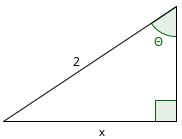
\includegraphics[width=0.25\textwidth]{./img/l2q4.png}
\end{figure}

Note que o cateto vertical pode ser expresso de duas maneiras, como a raiz da função dada inicialmente (se usarmos o teorema de pitágoras) ou em termos do $\sin(\theta)$. Como sabemos como integrar senos, vamos tentar usar essa ideia para uma troca de variáveis que nos ajude de fato.

\begin{questao}
Rescreva a integral $\int_{-2}^{2} \sqrt{4-x^2}dx$ usando a troca de variáveis $\sqrt{4-x^2}=\cos(\theta)$ (lembre-se que $x=2\sin(\theta)$).
\end{questao}

Não se esqueça de ajustar os limites da integral. Como $x=2\sin(\theta)$, e $x$ deve variar de $-2$ a $2$ a opção mais simples é variarmos $\theta$ de $-\pi/2$ a $\pi/2$. Portanto, nossa nova integral é:

$$\int_{-\pi/2}^{\pi/2} 2\cos(\theta). 2\cos(\theta)d\theta = 4 \int_{-\pi/2}^{\pi/2} \cos^2(\theta)d\theta$$

Nosso objetivo de obter uma integral que não envolve-se raízes foi atingido!

\subsection*{Pare e pense}

A transformação feita acima foi bem sucedida por um motivo: ao fazermos a troca $x=2\sin(\theta)$ também pudemos trocar a expressão $\sqrt{4-x^2}$ por $\cos(\theta)$. Vimos essa troca no triângulo, mas ela pode ser vista algebricamente graças à igualdade trigonométrica fundamental $\sin^2(\alpha) + \cos^2(\alpha)=1$. Ela implica que $\sin^2(\alpha)=1-\cos^2(\alpha)$. Portanto:

$$\sqrt{4-x^2} = \sqrt{4-4\sin^2(\theta)} = \sqrt{4-4(1-\cos^2(\theta))} = \sqrt{\cos^2(\theta)} = \cos(\theta)$$

Essa visão algébrica do processo é útil para que você possa aplicar essa troca em mais situações, não apenas naquelas que possam ser interpretadas em um triângulo retângulo. Por isso, o quadro abaixo traz as três variações da igualdade trigonométrica fundamental que lhe podem ser úteis.

\begin{shaded*}
$$\sin^2(\alpha) + \cos^2(\alpha)=1$$
$$\tan^2(\alpha) + 1= \sec^2(\alpha)$$
\end{shaded*}

Note que, na verdade, a segunda igualdade pode ser obtidas a partir da primeira, basta dividir todos os termos dela por $\cos^2(\alpha)$.

\begin{questao}
Considerando as igualdades acima:
\begin{enumerate}[a)]
\item Qual troca de variável você utilizaria se a função a ser integrada fosse $g(x)=\sqrt{1+x^2}$?
\item Como ficaria a integral $\int \sqrt{1+x^2} dx$ quando essa troca for completada?
\end{enumerate}
\end{questao}

\subsection*{Voltando à integral}

Antes da seção anterior, tínhamos chegado em $4\int_{-\pi/2}^{\pi/2} cos^2(\theta)d\theta$. Porém, mais uma vez, apesar da integral de $cos(\theta)$ ser simples, a de $cos^2(\theta)$ não é.

Se você tentar fazer a troca de variáveis $u=cos(\theta)$, vai notar que um seno aparecerá na expressão quando você transformar $d\theta$ em $du$. Esse problema é bastante comum quando integramos potências de seno e cosseno. O que pode ser feito para contornar essa dificuldade é utilizar uma outra família de igualdades trigonométricas. Talvez você as tenha estudado no Ensino Médio, caso não, sugerimos que memorize as duas igualdades mostradas abaixo:

\begin{shaded*}
$$\cos(2\alpha) = 2\cos^2(\alpha)-1$$
$$\sin(2\alpha) = 2\sin(\alpha).\cos(\alpha)$$
\end{shaded*}

Note que a primeira delas permite transformar um cosseno ao quadrado em um cosseno, enquanto que a segunda permite transformar um produto de seno por cosseno em um seno apenas. Essas igualdades são úteis para mudarmos o formato de potências de funções trigonométricas para formatos mais simles de integrar, como faremos agora.

Antes de retomarmos a integral, resolva a seguinte questão sobre as igualdades acima para que você se familiarize com o uso que será feito delas em MA111.

\begin{questao}
Considerando as igualdades acima:
\begin{enumerate}[a)]
\item Isole $\cos^2(\alpha)$ na primeira igualdade.
\item Use a igualdade $\sin^2(a) + \cos^2(a)=1$ e a resposta do item anterior para obter uma expressão que transforma $\sin^2(a)$ em $\cos(2a)$.
\item Rescreva a expressão $\sin^4(a)$ como uma expressão composta por senos e cossenos com as menores potências possíveis.
\end{enumerate}
\end{questao}

Note que a expressão obtida no item c acima pode parecer complicada, mas não envolve nenhuma potência e seria simples de integrar, ou seja, você fez quase todo o trabalho necessário para calcular $\int \sin^4(x)dx$.

Agora, voltemos à nossa integral.

\begin{questao}
Rescreva $4\int_{-\pi/2}^{\pi/2} cos^2(\theta)d\theta$, usando as igualdades anteriores, de modo que não haja mais potências no integrando.
\end{questao}

O que você fez na questão acima não é uma mudança de variável, mas sim uma manipulação algébrica que resultou em uma nova expressão equivalente à que tínhamos antes. Note que a expressão que você acabou de obter não tem mais cosseno ao quadrado e é simples de integrar.

\begin{questao}
Finalize essa questão calculando a integral obtida acima.
\end{questao}

Você deve ter obtido $2\pi$ como resposta, assim como havíamos adiantado no início.

\section{Mensagem final}

O grande objetivo deste capítulo era relembrar algumas identidades trigonométricas que são usadas com frequência quando utilizamos as técnicas de integração chamadas substituição trigonométrica e integrais trigonométricas.

A primeira família de igualdades (que derivam de $\sin^2(\alpha)+\cos^2(alpha)=1$) nos permitem:
\begin{enumerate}[1)]
\item Converter senos em cossenos, ou vice-versa;
\item Lidar com expressões do tipo $a^2-x^2$ fazendo a troca $x=\sin(\alpha)$;
\item Lidar com expressões do tipo $a^2+x^2$ fazendo a troca $x=\tan(\alpha)$.
\end{enumerate}

A segunda família de igualdades, envolvendo $\sin(2\alpha)$ e $\cos(2\alpha)$, nos permite:
\begin{enumerate}[1)]
\item Reduzir potências de funções trigonométricas para potências menores ($\cos^2(alpha)$ em $\cos(2\alpha)$), por exemplo;
\item Converter expressões produtos de senos e cossenos em expressões envolvendo $\sin(2\alpha)$.
\end{enumerate}

Sugerimos agora que você leia os exemplos 1, 2 e 3 da seção 7.2 do livro \sugestao{Calculus} e os exemplos 1, 2, 3 e 4 da seção 7.3. Em seguida, parta para a lista de exercícios da disciplina.

\newpage

\section{Gabarito}

Confira as respostas para as questões e \textbf{não se esqueça de registrar o seu progresso}.

\noindent\textbf{Questão 1:} a) $[-2;2]$, b) $-2$ e $2$, c) $(0;2)$, d) $[0;2]$.

\noindent\textbf{Questão 2:} a) circunferência de raio 2 e centro na origem.

\noindent\textbf{Questão 3:} a) a integral é igual à área de uma semi-circunferência de raio 2, b) $2\pi$.

\noindent\textbf{Questão 4:} $-2\int\sqrt{4u-u^2}du$

\noindent\textbf{Questão 5:} a) $\sqrt{4-x^2}$, b) $2\cos(\theta)$, c) $2\sin(\theta)$.

\noindent\textbf{Questão 6:} $4 \int_{-\pi/2}^{\pi/2} \cos^2(\theta)d\theta$.

\noindent\textbf{Questão 7:} a) $x=\tan(\alpha)$ e, portanto, $\sqrt(4+x^2)=\sec(\alpha)$, b) $\int \sec^3(\alpha)d\alpha$.

\noindent\textbf{Questão 8:} a) $\cos^2(\alpha)=\frac{\cos(2\alpha)+1}{2}$, b) $\sin^2(\alpha)=\frac{1-\cos(2\alpha)}{2}$, c) $\sin^4(\alpha)=\frac{1}{8} \cdot (3-4\cos(2\alpha)+\cos(4\alpha))$.


\section{Registro de progresso}

Essa parte por enquanto fica com conteúdo vazio até que seja decidido como será feito o controle do progresso.

\vspace{5cm}

\end{document}
